\section{Export}

Funcționalitatea de export a datelor dă utilizatorului ocazia de a scoate datele sale din aplicație și de a le valorifica în alte moduri mai complexe. La finalul procesului de export, utilizatorul are acces la un link de descărcare a bonurilor fiscale, arhivate în format \emph{p}. Figura \ref{exportForm} prezintă formularul pentru exportarea bonurilor. Opțiunile disponibile sunt:

\begin{itemize}
  \item
    \textbf{Conținut}: doar text sau text și imagine. Exportarea atât a datelor textuale, cât și a imaginilor conduce la un consum mai mare de date, de aceea este implementată și opțiunea \emph{doar text}. În cazul exportului imaginilor, fiecare obiect va conține un câmp cu numele imaginii aferente.
  \item
    \textbf{Format}: CSV sau JSON. Această opțiune oferă flexibilitate în disponibilitatea datelor. Formatul CSV exportă datele într-o manieră relațională, în două fișiere: \emph{transactions.csv} și \emph{products.csv}. Formatul JSON exportă un fișier pentru fiecare bon, ce conține datele tranzacției și o listă imbricată de produse.
  \item
    \textbf{Intervalul calendaristic}: Intervalul în care bonurule trebuie să se afle pentru a fi exportate.
\end{itemize}

\begin{figure}[ht]
  \centering
  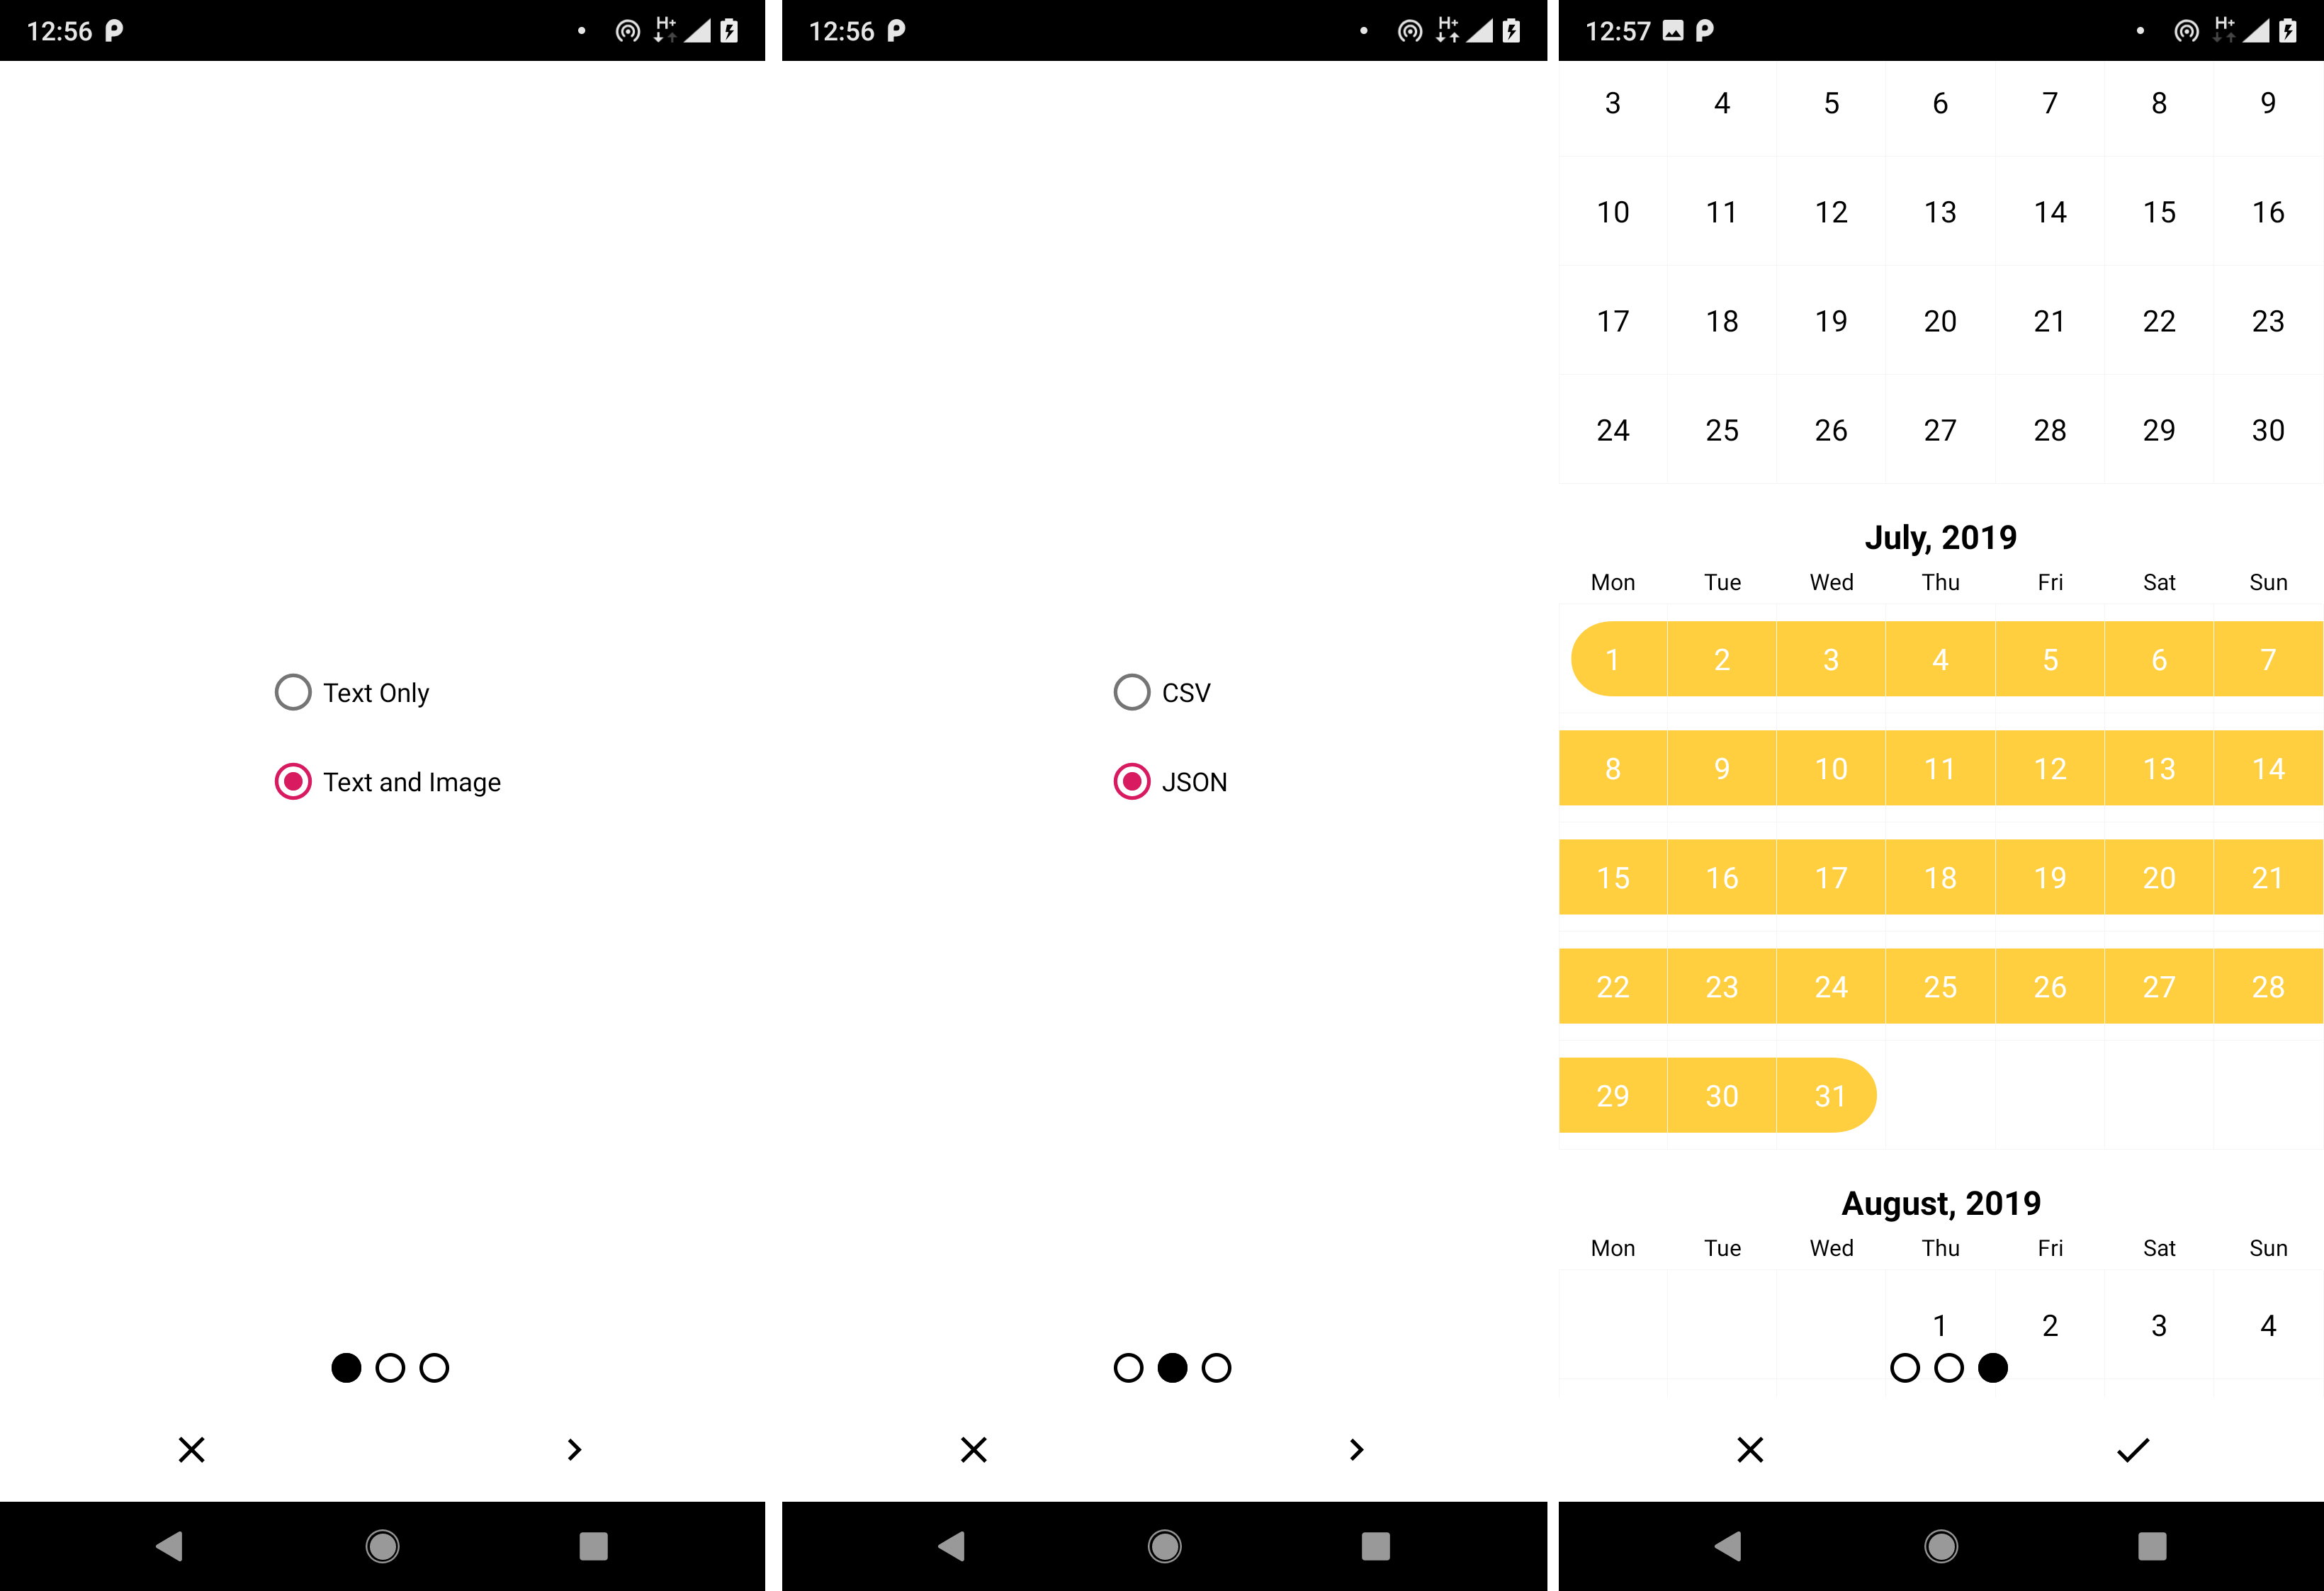
\includegraphics[width=\textwidth]{ExportForm.png}
  \caption{Formularul de export}
  \label{exportForm}
\end{figure}

Procesul de export funcționează în felul următor:

\begin{enumerate}
\item
  Utilizatorul completează formularul prezentat mai sus și datele exportului sunt salvate în baza de date locală cu statusul \emph{uploading}.
\item
  Aplicația afișează o notificare și trimite bonurile în cloud. La final, sesiunea de export este salvată cu statusul \emph{waiting download link}.
\item
  Bonurile sunt procesate în cloud pentru a fi trnsformate (în cazul în care formatul selectat a fost CSV) și arhivate.
\item
  Serviciul cloud trimite o notificare către dispozitiv ce conține \emph{link-ul} de descărcare a datelor. Acesta este salvat în baza de date locală, împreună cu statusul \emph{complete}.
\end{enumerate}

Figura \ref{exportsScreen} prezintă ecranul ce afișează export-urile utilizatorului. Un element conține intervalul calendaristic aferent exportului și statusul acestuia. Atunci când sesiunea de export este finalizată, două butoane sunt afișate, cu funcționalitatea de a copia link-ul de descărcare pe clipboard sau de a descărca datele arhivate pe dispozitiv.

\begin{figure}[ht]
  \centering
  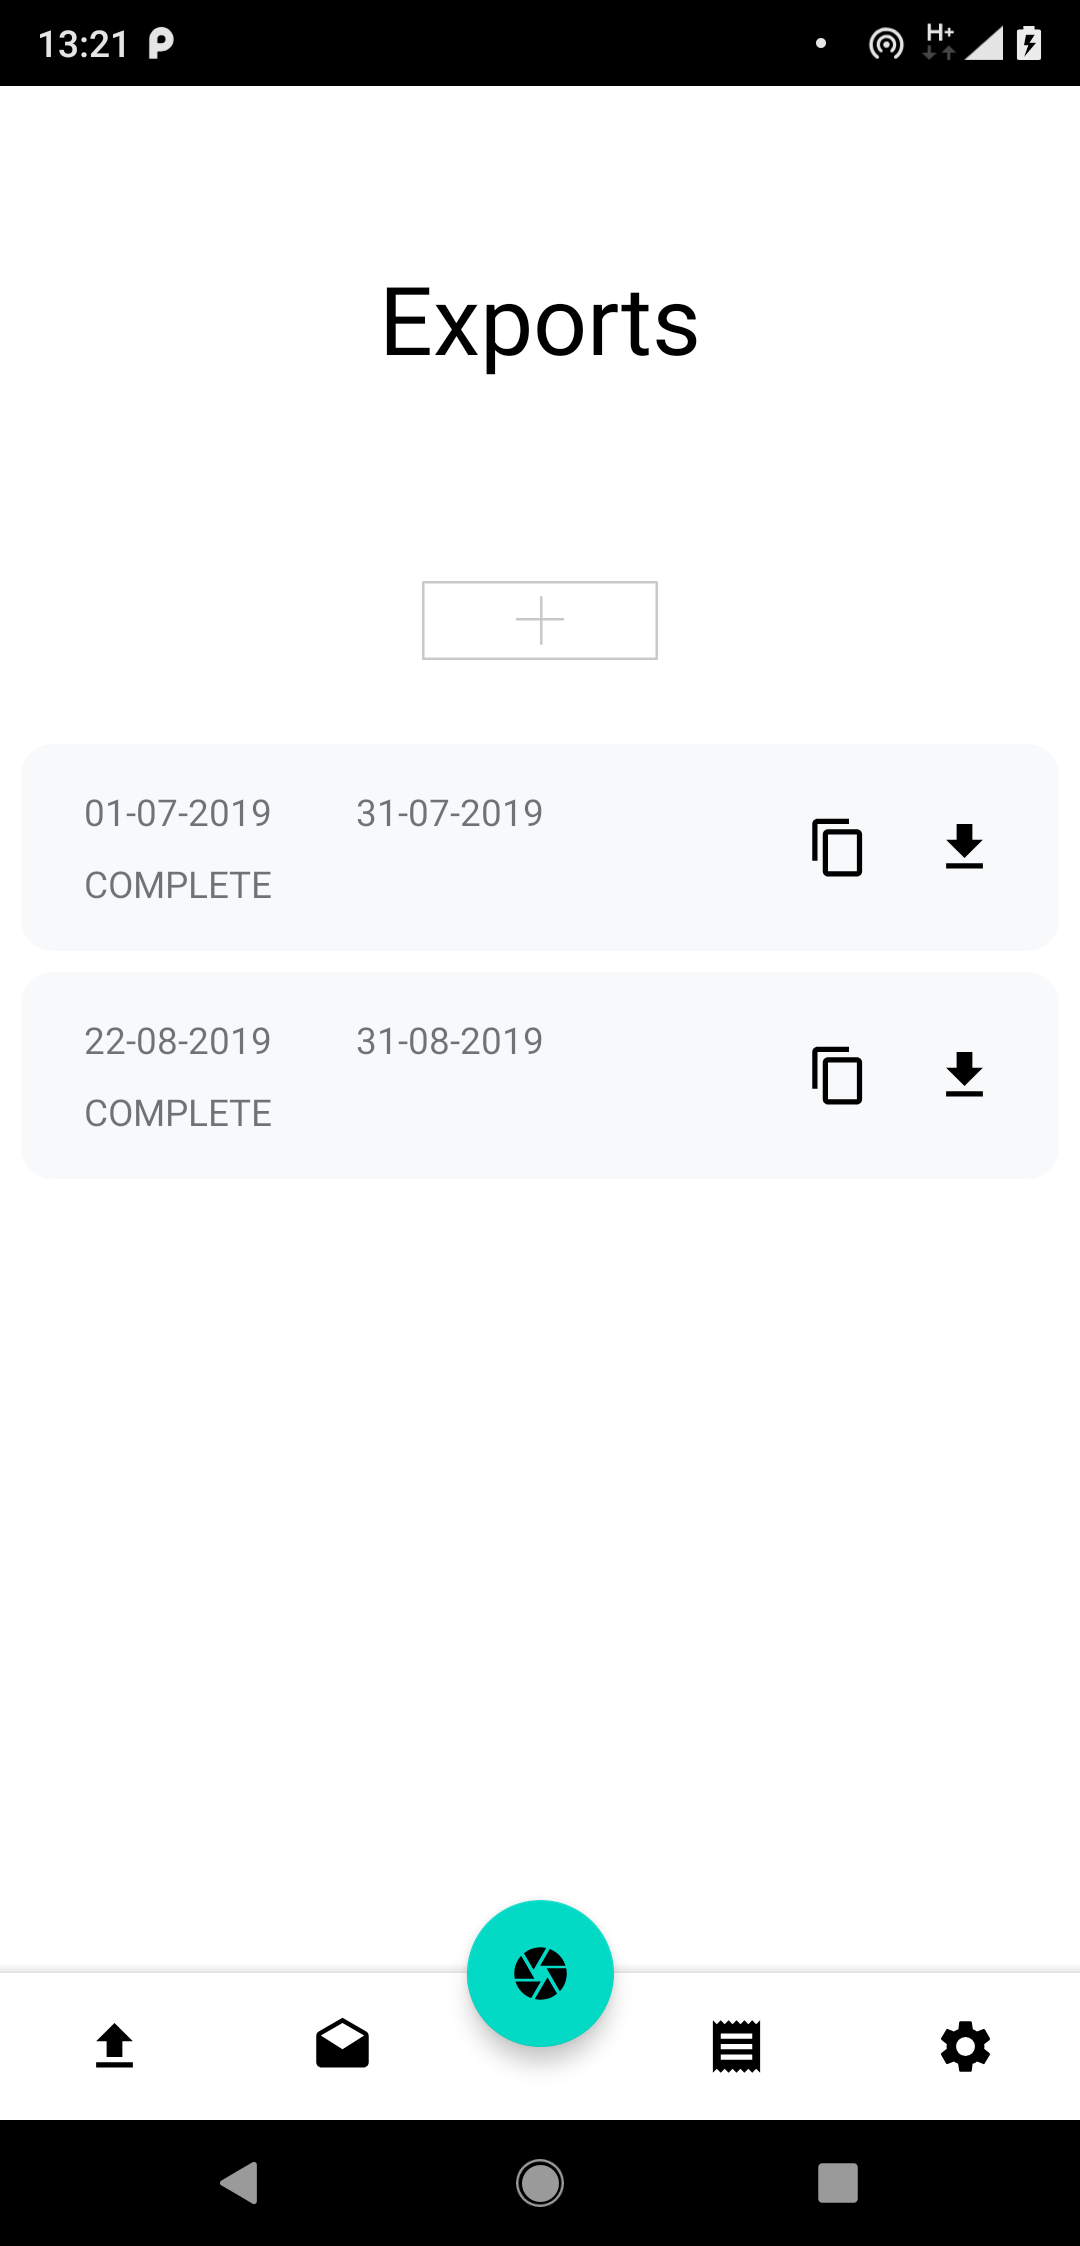
\includegraphics[width=\screenwidth]{ExportsScreen.png}
  \caption{Lista de export-uri}
  \label{exportsScreen}
\end{figure}

\subsection{Implementare}

La nivelul domeniului, funcționalitatea de export este modelată de interfața \texttt{ExportUseCase}. Aceasta definește funcțiile de listare a tuturor exporturilor de pe dispozitiv, creeare a unui nou export și marcarea unui export ca finalizat la primirea unei notificări.

\lstinputlisting[style=javaCodeStyle, caption=Interfața ExportUseCase]{./code/ExportUseCase.kt}

Trimiterea datelor către cloud se face printr-un serviciu de tipul \emph{foreground}. Pe sistemul Android, \emph{serviciile foreground} sunt servicii care interacționează cu utilizatorul prin intermediul unei notificări și au șanse foarte mici de a fi oprite de către sistem pentru a recupera resurse. Acestea sunt recomandate pentru a executa activități de lungă durată care nu blochează interfața și care sunt declanșate de o acțiune a utilizatorului. Funcția \texttt{upload} este apelată într-un astfel de serviciu cu argumentul obținut pe baza formularului prezentat mai sus. La creearea argumentului \texttt{Session} este generat un id unic ce va fi folosit pentru identificarea exportului pe durata funcționării acestuia.

Interacțiunea aplicației cu serviciile cloud Firebase pentru această funcționalitate este ilustrată în diagrama din figura \ref{exportProcess}.

\begin{figure}[ht]
  \centering
  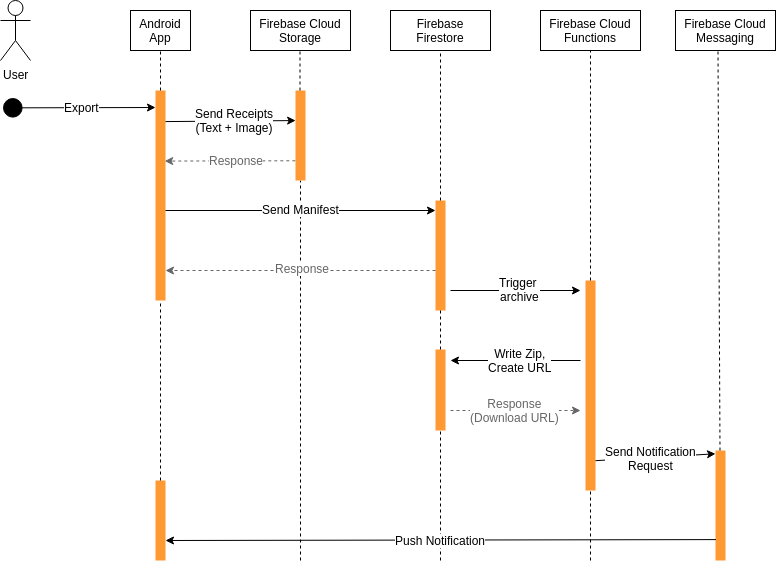
\includegraphics[width=\textwidth]{ExportSequence.png}
  \caption{Procesul de trimitere}
  \label{exportProcess}
\end{figure}

Serviciul de \emph{foreground} încarcă bonurile aferente exportului într-un spațiu de stocare \emph{Firebase Cloud Storage}, sub un folder ce are numele id-ului unic generat, în format JSON (opțional și imaginile JPEG respective). La încărcarea cu succes a acestor fișiere, obiectul \texttt{Session} este trimis ca manifest în colecția \emph{manifests} din serviciul \emph{Firebase Firestore}.

O funcție \emph{Firebase Cloud Functions} este configurată pentru a asculta modificări ale colecției \emph{manifests} și a se declanșa la creearea unui nou obiect. Aceasta citește id-ul manifestului și opțiunea de format (JSON sau CSV) și procesează fișierele din folder-ul corespunzător din \emph{Cloud Storage}. Apoi încarcă o arhivă \emph{zip} a acestui folder în folder-ul \emph{downloads} din Cloud Sotrage și generează un link de descărcare, pe care îl trimite către serviciul \emph{Firebase Cloud Messaging} pentru a fi trimis mai departe ca notificare către dispozitiv.

Pentru ca notificarea să ajungă doar la dispozitivul care a creeat exportul, aplicația folosește clientul Android al \emph{Firebase Cloud Messaging}. Acesta presupune implementarea unui serviciu ce extinde \texttt{FirebaseMessagingService}. Acest serviciu generează un \emph{token} folosit pentru a primi notificări și îl face disponibil în metoda \texttt{onNewToken(token:\ String)}. Aplicația salvează acest token în \emph{shared preferences} și îl trimite în obiectul manifest. Astfel, acest token ajunge pe cloud, de unde este transmis către \emph{Firebase Cloud Messaging}.

\emph{Firebase Cloud Messaging} suportă două tipuri de mesaje: \emph{notification messages} și \emph{data messages}, sau o combinație dintre cele două. (Firebase n.d.) Pentru ca notificarea să fie gestionată imediat ce a fost primită în metoda \texttt{onMessageReceived(message:\ RemoteMessage)} a serviciului \texttt{FirebaseMessagingService} este folosită doar funcționalitatea de \emph{data message}. Odată ce notificarea este recepționată de către dispozitiv, metoda \texttt{markAsFinished(notification:\ FinishedNotification)} este apelată pentru a actualiza baza de date și o notificare este afișată.

